\documentclass{beamer}
\let\vec\mathbf
\mode<presentation>
\usepackage{amsmath}
\usepackage{amssymb}
%\usepackage{advdate}
\usepackage{adjustbox}
%\usepackage{subcaption}
\usepackage{enumitem}
\usepackage{multicol}
\usepackage{mathtools}
\usepackage{listings}
\usepackage{url}
\usetheme{Boadilla}
\usecolortheme{lily}
\setbeamertemplate{footline}
{
  \leavevmode%
  \hbox{%
  \begin{beamercolorbox}[wd=\paperwidth,ht=2.25ex,dp=1ex,right]{author in head/foot}%
    \insertframenumber{} / \inserttotalframenumber\hspace*{2ex} 
  \end{beamercolorbox}}%
  \vskip0pt%
}
\setbeamertemplate{navigation symbols}{}
\providecommand{\nCr}[2]{\,^{#1}C_{#2}} % nCr
\providecommand{\nPr}[2]{\,^{#1}P_{#2}} % nPr
\providecommand{\mbf}{\mathbf}
\providecommand{\pr}[1]{\ensuremath{\Pr\left(#1\right)}}
\providecommand{\qfunc}[1]{\ensuremath{Q\left(#1\right)}}
\providecommand{\sbrak}[1]{\ensuremath{{}\left[#1\right]}}
\providecommand{\lsbrak}[1]{\ensuremath{{}\left[#1\right.}}
\providecommand{\rsbrak}[1]{\ensuremath{{}\left.#1\right]}}
\providecommand{\brak}[1]{\ensuremath{\left(#1\right)}}
\providecommand{\lbrak}[1]{\ensuremath{\left(#1\right.}}
\providecommand{\rbrak}[1]{\ensuremath{\left.#1\right)}}
\providecommand{\cbrak}[1]{\ensuremath{\left\{#1\right\}}}
\providecommand{\lcbrak}[1]{\ensuremath{\left\{#1\right.}}
\providecommand{\rcbrak}[1]{\ensuremath{\left.#1\right\}}}
\theoremstyle{remark}
\newtheorem{rem}{Remark}
\newcommand{\sgn}{\mathop{\mathrm{sgn}}}

\providecommand{\res}[1]{\Res\displaylimits_{#1}} 
\providecommand{\norm}[1]{\lVert#1\rVert}
\providecommand{\mtx}[1]{\mathbf{#1}}

\providecommand{\fourier}{\overset{\mathcal{F}}{ \rightleftharpoons}}
%\providecommand{\hilbert}{\overset{\mathcal{H}}{ \rightleftharpoons}}
\providecommand{\system}{\overset{\mathcal{H}}{ \longleftrightarrow}}
	%\newcommand{\solution}[2]{\textbf{Solution:}{#1}}
%\newcommand{\solution}{\noindent \textbf{Solution: }}
\providecommand{\dec}[2]{\ensuremath{\overset{#1}{\underset{#2}{\gtrless}}}}
\newcommand{\myvec}[1]{\ensuremath{\begin{pmatrix}#1\end{pmatrix}}}

\title{Matrices in Geometry - 4.3.24}
\author{EE25BTECH11035  Kushal B N}
\date{Sep, 2025}

\begin{document}

\maketitle

\section{Problem Statement}
\begin{frame}
\frametitle{Problem Statement}
Find the ratio in which the line $2x + 3y - 5 = 0$ divides the line segment joining the points $\brak{8,-9}$ and $\brak{2,1}$. Also find the coordinates of the point of division.
\end{frame}

\section{Solution}
\begin{frame}{Solution}
Given,\\
Line $\myvec{2 & 3}\myvec{x\\y} = 5$\\
Points $\vec{A}\myvec{8\\-9}$ and $\vec{B}\myvec{2\\1}$
Let $\vec{P}\myvec{h\\k}$ be the point on the given line dividing the line segment joining the given points. \\
So, the point $\vec{P}$ also lies on the line joining the given points $\vec{A}$ and $\vec{B}$.\\
The direction vector for this line would be\\
\begin{equation}
    \vec{d} = \vec{B} - \vec{A} = \myvec{-6\\10}
\end{equation}

So that the normal vector for the line(after dividing by common factor 2) will be\\
\begin{equation}
    \vec{n} = \myvec{5\\3}
\end{equation}
\end{frame}

\begin{frame}{Solution}
and in the line equation $\vec{n}^T\vec{P}=c$,\\
\begin{equation}
    c = \myvec{5&3}\myvec{2\\1} = 13
\end{equation}

Thus, the line equation is\\
\begin{equation}
    \myvec{5&3}\myvec{x\\y} = 13
\end{equation}

Solving for the intersection of the two lines, and by forming the augmented matrix,\\
\begin{equation}
    \myvec{2&3\\5&3}\myvec{x\\y} = \myvec{5\\13}
\end{equation}
\end{frame}

\begin{frame}{Solution}
\begin{equation}
    \implies \myvec{2&3&|&5\\5&3&|&13} \overset{R_1 \rightarrow \frac{1}{2}R_1}{\longrightarrow} \myvec{1&\frac{3}{2}&|&\frac{5}{2}\\5&3&|&13}
\end{equation}

\begin{equation}
    \myvec{1&\frac{3}{2}&|&\frac{5}{2}\\5&3&|&13} \overset{R_2 \rightarrow R_2 - 5R_1}{\longrightarrow} \myvec{1&\frac{3}{2}&|&\frac{5}{2}\\0&\frac{-9}{2}&|&\frac{1}{2}}
\end{equation}

\begin{equation}
    \myvec{1&\frac{3}{2}&|&\frac{5}{2}\\0&\frac{-9}{2}&|&\frac{1}{2}} \overset{R_2 \rightarrow \frac{-2}{9}R_2}{\longrightarrow} \myvec{1&\frac{3}{2}&|&\frac{5}{2}\\0&1&|&\frac{-1}{9}} 
\end{equation}

\begin{equation}
    \implies \vec{P} = \myvec{\frac{8}{3}\\ \frac{-1}{9}}
\end{equation}

\end{frame}

\begin{frame}{Solution}
Section Formula for a point $\vec{P}$ which divides the line segment formed by points $\vec{A}$ and $\vec{B}$ in the ratio $k:1$ is given by\\
\begin{equation}
    \vec{P} = \frac{k\vec{B}+\vec{A}}{k+1}
\end{equation}

\begin{equation}
    k\brak{\vec{P}-\vec{B}} = \vec{A} - \vec{P}
\end{equation}

\begin{equation}
    \implies k = \frac{\brak{\vec{A}-\vec{P}}^{\top}\brak{\vec{P}-\vec{B}}}{\norm{\vec{P}-\vec{B}}^2}
\end{equation}

\begin{equation}
    \brak{{\vec{A}-\vec{P}}}^{\top}\brak{\vec{P}-\vec{B}} = \myvec{\frac{16}{3}&\frac{-80}{9}}\myvec{\frac{2}{3}\\ \frac{-10}{9}} = \frac{1088}{81}
\end{equation}

\begin{equation}
    {\norm{\vec{P}-\vec{B}}}^2 = \brak{\vec{P}-\vec{B}}^{\top}\brak{\vec{P}-\vec{B}} = \frac{136}{81}
\end{equation}

\begin{equation}
    \implies \fbox{k=8}
\end{equation}
\end{frame}

\section{Conclusion}
\begin{frame}{Conclusion}
$\therefore$ The ratio in which the line divides the two given points is 8:1 and the coordinates of the point of division is $\myvec{\frac{8}{3}\\ \frac{-1}{9}}$.

\begin{figure}
    \centering
    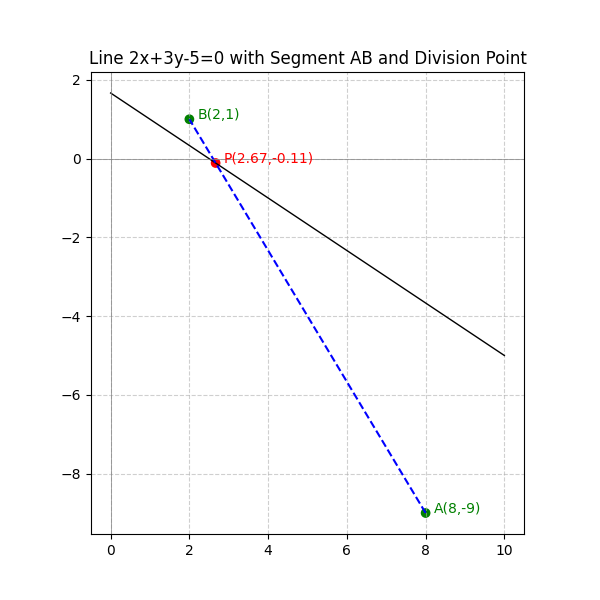
\includegraphics[width=0.55\columnwidth]{figs/2.png}
    \caption{}
    \label{fig:placeholder}
\end{figure}
\end{frame}
\end{document}

